%==============================================================================
% Sjabloon onderzoeksvoorstel bachelorproef
%==============================================================================
% Gebaseerd op LaTeX-sjabloon ‘Stylish Article’ (zie voorstel.cls)
% Auteur: Jens Buysse, Bert Van Vreckem

\documentclass[fleqn,10pt]{voorstel}

%------------------------------------------------------------------------------
% Metadata over het voorstel
%------------------------------------------------------------------------------

\JournalInfo{HoGent Bedrijf en Organisatie}
\Archive{Bachelorproef 2018 - 2019} % Of: Onderzoekstechnieken

%---------- Titel & auteur ----------------------------------------------------

% TODO: geef werktitel van je eigen voorstel op
\PaperTitle{Virtual reality als sleutel tot succesvolle revalidatie}
\PaperType{Onderzoeksvoorstel Bachelorproef} % Type document

% TODO: vul je eigen naam in als auteur, geef ook je emailadres mee!
\Authors{Bruno Stroobants\textsuperscript{1}} % Authors
\CoPromotor/
\affiliation{\textbf{Contact:}
  \textsuperscript{1} \href{mailto:bruno.stroobants.y9084@student.hogent.be}{bruno.stroobants.y9084@student.hogent.be};
  \textsuperscript{2}
}

%---------- Abstract ----------------------------------------------------------

\Abstract{
    Tijdens deze scriptie wordt onderzocht wat de gevolgen zijn van virtual reality in het revalidatieproces van mensen die moeite hebben met het consistent uitvoeren van opgelegde oefeningen door de kinesist. Velen zijn niet genoeg gemotiveerd om dagelijks saaie, repetitieve oefeningen te verrichten. Dit heeft natuurlijk een negatieve impact op hun revalidatie en daarom is er hiervoor een oplossing nodig. Tijdens het onderzoek zal er een applicatie ontwikkeld worden voor een VR platform. Deze applicatie zal de patiënt op een interactieve en speelse manier bijstaan bij het uitvoeren van de opgelegde oefeningen. Vervolgens zal de applicatie in de praktijk getest worden en er zal onderzocht worden of men op deze wijze de patiënt kan motiveren. Er wordt verwacht dat deze manier van werken zeker zal aanslaan bij de jongere patiënten en tevens resultaat zal kennen bij de gemiddelde volwassene patiënten.
}

%---------- Onderzoeksdomein en sleutelwoorden --------------------------------
% TODO: Sleutelwoorden:
%
% Het eerste sleutelwoord beschrijft het onderzoeksdomein. Je kan kiezen uit
% deze lijst:
%
% - Mobiele applicatieontwikkeling
% - Webapplicatieontwikkeling
% - Applicatieontwikkeling (andere)
% - Systeembeheer
% - Netwerkbeheer
% - Mainframe
% - E-business
% - Databanken en big data
% - Machineleertechnieken en kunstmatige intelligentie
% - Andere (specifieer)
%
% De andere sleutelwoorden zijn vrij te kiezen

\Keywords{Applicatieontwikkeling. Virtuele realiteit --- Kinesitherapie --- Revalidatie} % Keywords
\newcommand{\keywordname}{Sleutelwoorden} % Defines the keywords heading name

%---------- Titel, inhoud -----------------------------------------------------

\begin{document}

\flushbottom % Makes all text pages the same height
\maketitle % Print the title and abstract box
\tableofcontents % Print the contents section
\thispagestyle{empty} % Removes page numbering from the first page

%------------------------------------------------------------------------------
% Hoofdtekst
%------------------------------------------------------------------------------

% De hoofdtekst van het voorstel zit in een apart bestand, zodat het makkelijk
% kan opgenomen worden in de bijlagen van de bachelorproef zelf.
%---------- Inleiding ---------------------------------------------------------

\section{Introductie} % The \section*{} command stops section numbering
\label{sec:introductie}

In dit onderzoek gaan we na of virtuele realiteit als hulpmiddel kan fungeren bij de revalidatie van kinesitherapie patiënten en welke mogelijke voordelen het zou hebben. Vele patiënten voeren hun revalidatie oefeningen uit met tegenzin omdat ze vaak saai en repetitief kunnen zijn. Een gevolg hiervan is dat sommigen wel eens een oefensessie overslaan. Een heus probleem in de revalidatiesector dus dat we trachten te onderzoeken en mogelijks kunnen verbeteren of zelfs oplossen.


%---------- Stand van zaken ---------------------------------------------------

\section{State of the art}
\label{sec:start-of-the-art}

\subsection{Literatuurstudie}
Tijdens mijn literatuurstudie stootte ik vooral op artikels deels gelijkaardig aan mijn onderwerp, nl. over het gebruik van virtuele realiteit bij revalidatie na een beroerte. Vele artikels hierover waren echter reeds verouderd. Een interessant artikel dat ik vond was dat van \textcite{Laver2017}. Hier werd een behandeling op basis van virtuele realiteit vergeleken met de traditionele behandeling na een beroerte. In dit onderzoek keek men naar drie verschillende criteria: de armfunctie, de loopsnelheid en de mate waarin de patiënt zelfstandig alledaagse activiteiten kon voltooien. Er werden echter geen significante verschillen aangetroffen tussen beide methoden. In een ander artikel \textcite{Boian2002} werden ook patiënten die een beroerte opgelopen hadden onderzocht. Hier stond de revalidatie van de handen centraal. De patiënten kregen een virtuele applicatie voorgeschoteld waar ze objecten moesten oppakken e.d. Uit het onderzoek bleek vervolgens dat het bewegingsbereik van de vingers uitgebreid was.  Vervolgens vond ik ook een artikel \textcite{Reddy2018} dat zich handelt over hoe virtuele realiteit momenteel al vaak wordt ingezet in de psychiatrie om angststoornissen te bestrijden. Hier wordt de patiënt stapsgewijs aan zijn angst blootgesteld in een veilige omgeving en leert hij er langzamerhand mee omgaan. Er gebeurden in het verleden dus al enkele gelijkaardige onderzoeken naar virtuele realiteit in de gezondheidszorg maar nog niet bepaald in de richting waar ik op wil gaan.

\subsection{Bestaande applicaties}
Op mijn zoektoch in het onderzoeksdomein leerde ik een bedrijf kennen genaamd KineQuantum. Dit is een bedrijf dat zich specialiseert in het maken van een VR-applicatie die patiënten bijstaat bij het revalideren. In deze applicatie zitten de patiënten volledig in een virtuele wereld waar ze allerlei oefeningen moeten uitvoeren terwijl de kinesist nog steeds de mogelijkheid heeft om de patiënt op te volgen. Ook wordt de vooruitgang automatisch opgeslagen en deze kan ook geraadpleegd worden door de dokter.
%---------- Methodologie ------------------------------------------------------
\section{Methodologie}
\label{sec:methodologie}

In de onderzoeksfase zal ik nagaan welk VR platform het meest geschikt zou zijn voor het onderzoek. Hierna zal ik een applicatie ontwikkelen voor het gekozen platform waarin de gebruiker op een interactieve, speelse manier bepaalde handelingen moet uitvoeren. In de praktijk zal ik de applicatie vervolgens laten testen door meerdere patiënten. Na de demo zal ik hen een vragenlijst voorleggen om te bepalen wat ze er zelf van vonden.



%---------- Verwachte resultaten ----------------------------------------------
\section{Verwachte resultaten}
\label{sec:verwachte_resultaten}

\begin{figure}[h]
    \centering
    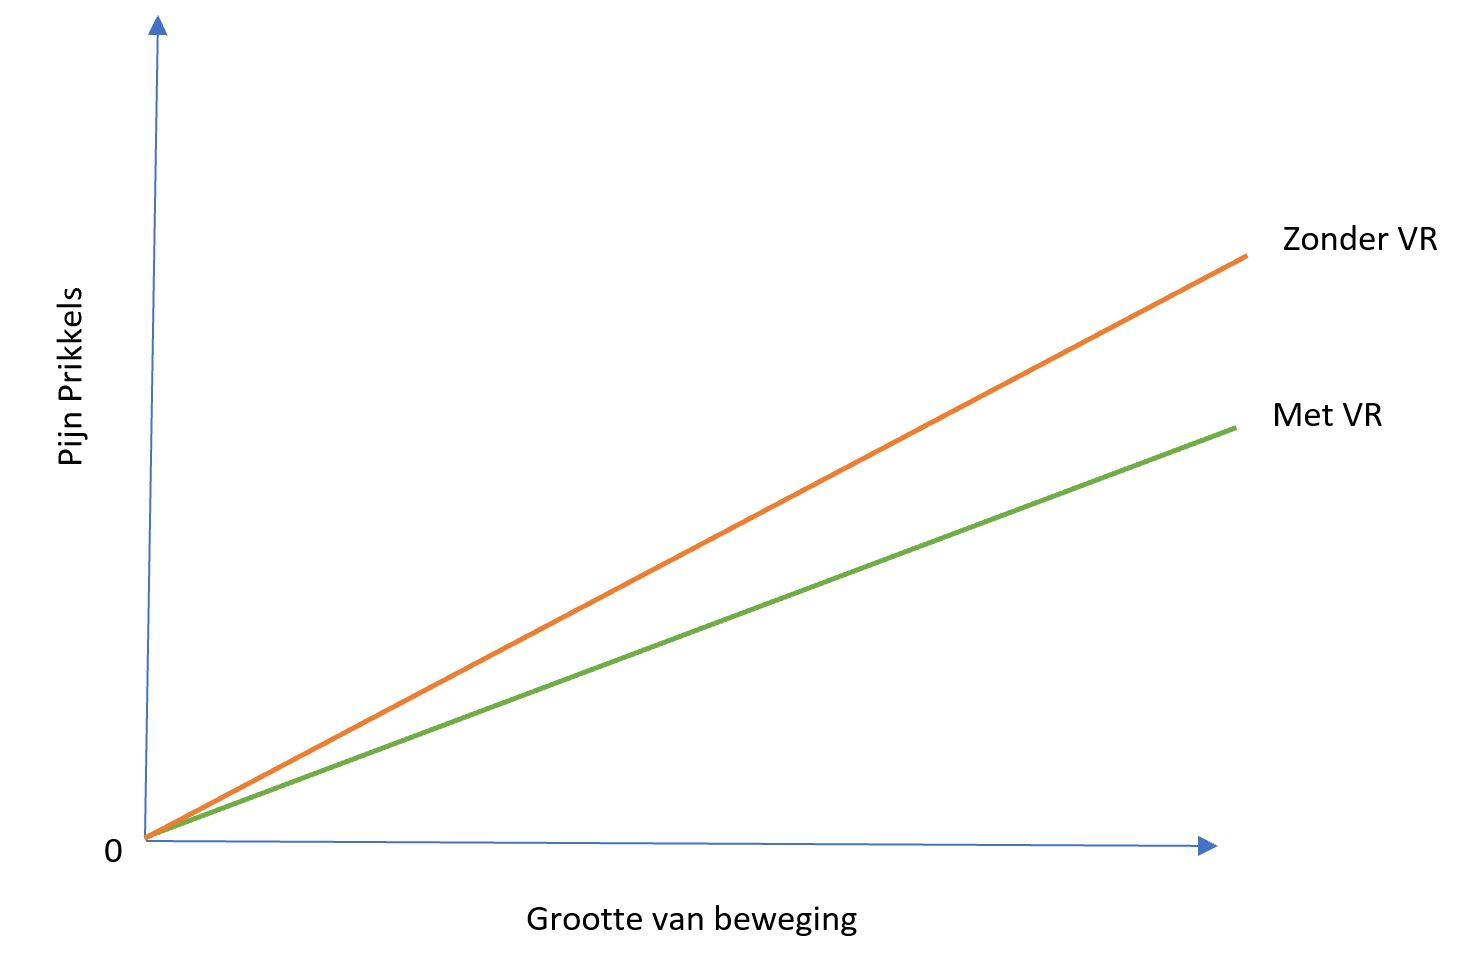
\includegraphics[scale=0.5]{mockupGraph.JPG}
    \caption{Mock-up grafiek}
    \label{graph}
\end{figure}



%---------- Verwachte conclusies ----------------------------------------------
\section{Verwachte conclusies}
\label{sec:verwachte_conclusies}

Ik denk dat een dergelijke manier van revalideren zeker zal aanslaan bij de patiënten en het hen meer zal motiveren om hun oefeningen consistent uit te voeren. Ook denk ik dat de virtuele omgeving een positief effect zal hebben op de pijnprikkels en dat men sneller resultaten zal boeken op vlak van revalidatie. 




%------------------------------------------------------------------------------
% Referentielijst
%------------------------------------------------------------------------------
% TODO: de gerefereerde werken moeten in BibTeX-bestand ``voorstel.bib''
% voorkomen. Gebruik JabRef om je bibliografie bij te houden en vergeet niet
% om compatibiliteit met Biber/BibLaTeX aan te zetten (File > Switch to
% BibLaTeX mode)

\phantomsection
\printbibliography[heading=bibintoc]

\end{document}
